%% IEEE Robotics and Automation Letters (RA-L) Template
%% IEEEtran class, two-column, 6 pages max (excl. references)
%%
%% Project: Napoleon2025 — Embodied Autonomous Bronchoscope
%% Author: Z.Q.   Draft v1.0   2026-07-02
%% Status: Full manuscript, experimental numbers to be filled after phantom trials.

\documentclass[journal,comsoc]{IEEEtran}

% ── Packages ────────────────────────────────────────────────────
\usepackage[T1]{fontenc}
\usepackage[utf8]{inputenc}
\usepackage{amsmath,amssymb,amsfonts}
\usepackage{algorithm}
\usepackage{algpseudocode}
\usepackage{graphicx}
\usepackage{booktabs}
\usepackage{multirow}
\usepackage{xcolor}
\usepackage{hyperref}
\usepackage{cite}
\usepackage{url}
\usepackage{subcaption}
\usepackage{balance}   % balance last-page columns
\usepackage{enumitem} % tighter itemize spacing

% ── Macros ──────────────────────────────────────────────────────
\newcommand{\TODO}[1]{\textcolor{red}{\textbf{[TODO: #1]}}}
\newcommand{\Tobs}{T_{\text{obs}}}
\newcommand{\dobs}{d_{\text{obs}}}
\newcommand{\Ngoal}{N_{\text{goal}}}
\newcommand{\obs}{\mathbf{o}}
\newcommand{\act}{\mathbf{a}}
\newcommand{\hid}{\mathbf{h}}
\newcommand{\goal}{g}
\newcommand{\embg}{\mathbf{e}_{g}}

% ── Title ───────────────────────────────────────────────────────
\title{An Embodied Autonomous Bronchoscope Platform with\\
Multimodal Perception and Goal-Conditioned Imitation Learning}

\author{%
  Z.~Qian,~\IEEEmembership{Graduate~Student~Member,~IEEE},
  Z.~Li,~\IEEEmembership{Member,~IEEE},
  and~H.~Ren,~\IEEEmembership{Senior~Member,~IEEE}%
  \thanks{Manuscript received July 2, 2026; revised \TODO{XX\,\,XX, 2026}.}%
  \thanks{This work was supported by the Ph.D.\ research fund of the
          corresponding author and the Medical Robotics Laboratory
          at \TODO{Affiliation~1}.}
  \thanks{Z.~Qian is with the Department of Biomedical Engineering,
          \TODO{Affiliation~1}, City, Country (e-mail: \TODO{author@email}).}%
  \thanks{Z.~Li and H.~Ren are with the Department of Mechanical
          Engineering, \TODO{Affiliation~1}, City, Country.}}
\markboth{IEEE Robotics and Automation Letters,~Vol.~\TODO{X},~No.~\TODO{X},~\TODO{Month}~\TODO{Year}}%
{Z.~Qian \MakeLowercase{\textit{et al.}}: Embodied Autonomous Bronchoscope}

% ── Begin Document ──────────────────────────────────────────────
\begin{document}

\maketitle

% ── Abstract ────────────────────────────────────────────────────
\begin{abstract}
We present an embodied autonomous bronchoscope platform that integrates
multimodal perception with goal-conditioned behavior cloning for
real-time (20\,Hz) navigation across the bronchial tree and
mucus-obstruction clearance. A unified 20-dimensional structured
observation vector fuses real-time semantic segmentation (UNet),
metric depth estimates (Depth-Anything-V2 with a ViT-L encoder), and
a depth-guided three-column path analyser (DepthPathFinder) with
motor proprioception. A goal-conditioned gated recurrent unit network
(\textit{BronchusPolicy}) with an auxiliary subtask-classification
head maps an eight-frame observation window and a discrete anatomical
target token ($\goal\!\in\!\{0,\dots,9\}$, ten paths including
exploration) to three-degree-of-freedom motor increments, achieving
$\approx$\,0.4\,M parameters and $<$5\,ms wall-clock inference on an
RTX~3090. A state-machine-driven autonomous controller layers an
average-trajectory playback, a vision-based junction corrector, and an
obstruction handler with checkpoint-and-return; expert demonstrations
at 20\,Hz are recorded to HDF5 directly during teleoperation.
We benchmark the system against a reactive visual-servoing baseline
on a 3-D-printed bronchial phantom and outline a forthcoming
ex-vivo porcine lung evaluation. Initial results indicate a
navigation success rate in the \TODO{XX--XX}\,\% range with mean
endpoint error of \TODO{XX}\,mm, demonstrating that a single
lightweight policy can serve multi-pathway goal-directed navigation
on a real robotic bronchoscope.
\end{abstract}

\begin{IEEEkeywords}
Autonomous bronchoscopy, behavior cloning, multimodal perception,
depth foundation model, goal-conditioned policy, medical robotics,
imitation learning.
\end{IEEEkeywords}

% ── I. Introduction ─────────────────────────────────────────────
\section{Introduction}
\label{sec:intro}

Flexible bronchoscopy is the gold-standard diagnostic and therapeutic
procedure for airway inspection, biopsy, and mucus clearance in
patients with pulmonary disease. Manual navigation of a flexible
bronchoscope through the highly branched tracheobronchial tree
demands years of training to coordinate real-time endoscopic imagery
with instrument-tip deflection; operator fatigue and inter-clinician
variability remain pressing concerns, particularly in intensive-care
settings where repeated bronchial toilet is required.

\paragraph{Robotic bronchoscopy is now clinical, but not autonomous.}
Robotic bronchoscopy has matured to clinical use, as demonstrated by
the Monarch platform (Auris/J\&J)\cite{target2025}---whose TARGET
study reported lesion reach in 98.7\% of cases (679 patients,
21 sites)---and the Ion Endoluminal System (Intuitive)\cite{target2025}.
Both platforms, however, still require the operator to select every
bifurcation turn manually; full waypoint autonomy remains an open
problem. The key open challenges are: (i)~robust lumen and bifurcation
perception in the textureless, specular, wet endoscopic environment;
(ii)~bifurcation-aware path selection under anatomical variability;
and (iii)~learning-based policies that generalise without requiring an
accurate kinematic model of the flexible instrument.

\paragraph{Recent vision foundation models and visuomotor policies
create new opportunities.}
Two threads of progress are converging. First, monocular depth
foundation models \textit{Depth~Anything~V2}~(DAM-V2)
\cite{yang2024depthv2,oquab2023dinov2}, combined with parameter-efficient
adaptation techniques (\textit{DARES} \cite{dares2024},
\textit{EndoDAC}\cite{endodac2024}, \textit{MonoLoT}\cite{monolot2024},
\textit{DAE}\cite{longshort2026}), now achieve metric-grade depth on
endoscopic video with sub-30\,ms latency. Second, recurrent and
diffusion-based visuomotor policies
\cite{cho2014gru,chi2023diffusion,zhao2023act} have demonstrated
end-to-end image-to-action mapping in manipulation and a few flexible
endoscopy tasks. Yet in clinical bronchoscopy, end-to-end policies
have so far only been demonstrated in simulation
\cite{pore2024bronchocopilot,zhang2024aicopilot} or in highly
specialised vision-only architectures
\cite{longshort2026}.

\paragraph{Contributions.}
In this letter we close the gap between simulated end-to-end policies
and clinical robotics. Our contributions are:

\begin{enumerate}[leftmargin=*,topsep=2pt,itemsep=0pt]
  \item \textbf{A unified multimodal-perception pipeline for
        bronchoscopy.} UNet (VGG-16) segmentation,
        Depth-Anything-V2 metric depth, and the three-column
        DepthPathFinder are fused into a compact 20-dimensional
        observation vector that captures lumen geometry, bifurcation
        topology, mucus location, and instrument proprioception.
        The pipeline runs synchronously at the 20\,Hz motor loop.
  \item \textbf{A goal-conditioned GRU policy with dual-head training
        (\textit{BronchusPolicy}).} A 0.4\,M-parameter recurrent
        network maps an eight-frame observation window and a
        discrete anatomical target token
        ($\goal\!\in\!\{0,\dots,9\}$) to motor-increment
        predictions and a subtask (navigate/clear) decision under a
        joint MSE + cross-entropy objective.
  \item \textbf{A hierarchical autonomous controller on a real robotic
        bronchoscope.} An average-trajectory playback with junction
        correction and obstruction handling with checkpoint-and-return
        state machine runs on a \TODO{3-DoF} RMD-motor bronchoscope
        in real time (20\,Hz) with voice-driven user-interface.
  \item \textbf{Initial phantom validation with a planned ex-vivo
        study.} Quantitative metrics (NSR, MEE, jerk, latency) are
        benchmarked against a reactive visual-servoing baseline,
        with a planned extension to ex-vivo porcine lung.
\end{enumerate}

\paragraph{Comparison with concurrent work.}
\emph{AI co-pilot}~\cite{zhang2024aicopilot} trains an imitation
policy in a CT-derived simulator with DAgger aggregation and maps five
discrete teleoperator regions to actions; although elegant in
sim-to-real, it is anchored to a simulated expert. \emph{BronchoCopilot}
\cite{pore2024bronchocopilot} uses multimodal RL with auxiliary
reconstruction, but it is evaluated only in simulation and reports
fifth-generation airways. \emph{Long-Short Term Agents}
\cite{longshort2026} adopt a hierarchical ``world-model critic''
architecture that predicts visual states at ambiguous branch points and
have achieved 80\,\% success to the eighth generation on ex-vivo
porcine lung. Our work complements these by (a)~fusing depth and
segmentation rather than relying on visual servoing alone, (b) using
a single lightweight recurrent network across ten target tokens
(including exploration), and (c)~relying entirely on
real-robot expert demonstrations rather than simulated experts.

% ── II. Related Work ────────────────────────────────────────────
\section{Related Work}
\label{sec:related}

\subsection{Robotic Bronchoscopy Platforms}
Tendon-driven continuum manipulators provide the mechanical basis for
flexible bronchoscopy \cite{camarillo2008mechanics,roesthuis2014continuum},
yet their non-holonomic kinematics and rate-dependent hysteresis
substantially complicate analytic control \cite{cho2024hysteresis}.
Two commercial systems are now clinically deployed: the \emph{Monarch}
platform (Auris / Johnson \& Johnson), whose TARGET trial
demonstrated 98.7\,\% lesion reach and 83.2\,\% diagnostic yield
\cite{target2025}, and Intuitive's \emph{Ion} Endoluminal System with
its 3.5\,mm shape-sensing catheter \cite{target2025}. Both platforms
require continuous teleoperator guidance; to the best of our knowledge
neither yet supports fully autonomous waypoint navigation.
Recent patient-mounted reconfigurable platforms further push the
miniaturisation frontier \cite{lawson2024assembled}.

\subsection{Endoscopic and Bronchoscopic Perception}
Self- and weakly-supervised depth estimation in endoscopy is being
transformed by vision foundation models. DAM-V2 \cite{yang2024depthv2}
delivers metric depth on diverse scenes, and surgical-adaptation
methods (\textit{DARES}\cite{dares2024}, \textit{EndoDAC}
\cite{endodac2024}, \textit{MonoLoT}\cite{monolot2024}) close the
domain gap with parameter-efficient LoRA-style adapters. For
bronchial carina detection, deep learning replaces rule-based
region-growing pipelines \cite{faia240657,naviairway2022}, while
landmark datasets such as BM-BronchoLC \cite{bm-broncholc2024}
catalogue anatomical variations. We adopt DAM-V2 with a
validity-gate and a temporal-jump filter and combine it with the
UNet semantic segmentation in a single 20-dim observation vector.

\subsection{Visuomotor Policy Learning}
Behavior cloning (BC) and its offline variants remain a strong
baseline for visuomotor control
\cite{ross2011dagger,ho2016gail,cho2014gru}. Recurrent
GRU-based policies handle partial observability in sequential
navigation \cite{chi2023diffusion,zhao2023act}, while diffusion-based
and action-chunking transformers have surpassed LSTM baselines in
manipulation \cite{chi2023diffusion,zhao2023act}; 3-D diffusion
policies such as DP3 \cite{ze2024dp3} extend generalisation with
point-cloud inputs. Vision-Language-Action (VLA) models
\cite{kim2024openvla} support language-conditioned generalisation
but currently require substantial compute and data. For our 20\,Hz
real-time budget and a 0.4\,M-parameter footprint, the dual-head GRU
remains the most appropriate trade-off.

\subsection{Autonomous Endoscopy and Bronchoscopy}
Visual-servoing approaches dominate colon navigation. Li \emph{et~al.}
\cite{li2024east,li2024polyp} combine deep-learning contour with
``darkest-region'' heuristics to drive an electromagnetically
actuated soft-tethered colonoscope in a phantom and ex-vivo colon,
reducing operator workload but without learned policies. Reinforcement
learning has been explored for digestive endoscopy with human
intervention (\textit{HI-PPO}) and follow-the-leader architectures
\cite{pore2024hi}. Closest to our setting are two simulation-only
methods: \emph{AI co-pilot}~\cite{zhang2024aicopilot} uses
imitation learning in a CT-derived simulator with DAgger aggregation,
and \emph{BronchoCopilot}~\cite{pore2024bronchocopilot} reports
$\sim$90\,\% success on fifth-generation airways via multimodal RL.
On real hardware, the vision-only hierarchical policy of
\cite{longshort2026} achieved 80\,\% success to the eighth generation
ex-vivo. Our work differs in (i)~fusing segment+depth+proprioception
into a 20-dim observation rather than relying on a single modality;
(ii)~training on real-robot demonstrations rather than in simulation;
and (iii)~supporting a single recurrent policy across ten anatomical
targets.

\begin{table}[t]
\caption{Summary of representative navigation methods for
flexible endoscopes. \emph{Real-phantom} and
\emph{real-ex-vivo/in-vivo} indicate physical experiments.}
\label{tab:related}
\centering
\small
\begin{tabular}{lcccl}
\toprule
Method & Sensor & Policy & Eval. setting & Reported NSR (\%)\\
\midrule
Li \textit{et al.} \cite{li2024east} &
  RGB (DL lumen) &
  Reactive servoing &
  Phantom + ex-vivo (colon) &
  \TODO{XX}\\
BronchoCopilot \cite{pore2024bronchocopilot} &
  RGB + pose &
  Multimodal RL &
  Simulation only &
  $\sim$90 (5th gen)\\
AI co-pilot \cite{zhang2024aicopilot} &
  RGB &
  BC + DAgger (Sim2Real) &
  Real ex-vivo (porcine) &
  \TODO{XX}\\
Long-Short Agents \cite{longshort2026} &
  RGB &
  World-model critic &
  Phantom + ex-vivo + in-vivo &
  100/80/\TODO{XX}\\
\textbf{Ours (this work)} &
  \textbf{RGB+depth+seg+proprio.} &
  \textbf{Goal-cond.\ GRU} &
  \textbf{Phantom (planned: ex-vivo)} &
  \TODO{XX}\\
\bottomrule
\end{tabular}
\end{table}

% ── III. System Overview ────────────────────────────────────────
\section{System Overview}
\label{sec:system}

\begin{figure}[t]
  \centering
  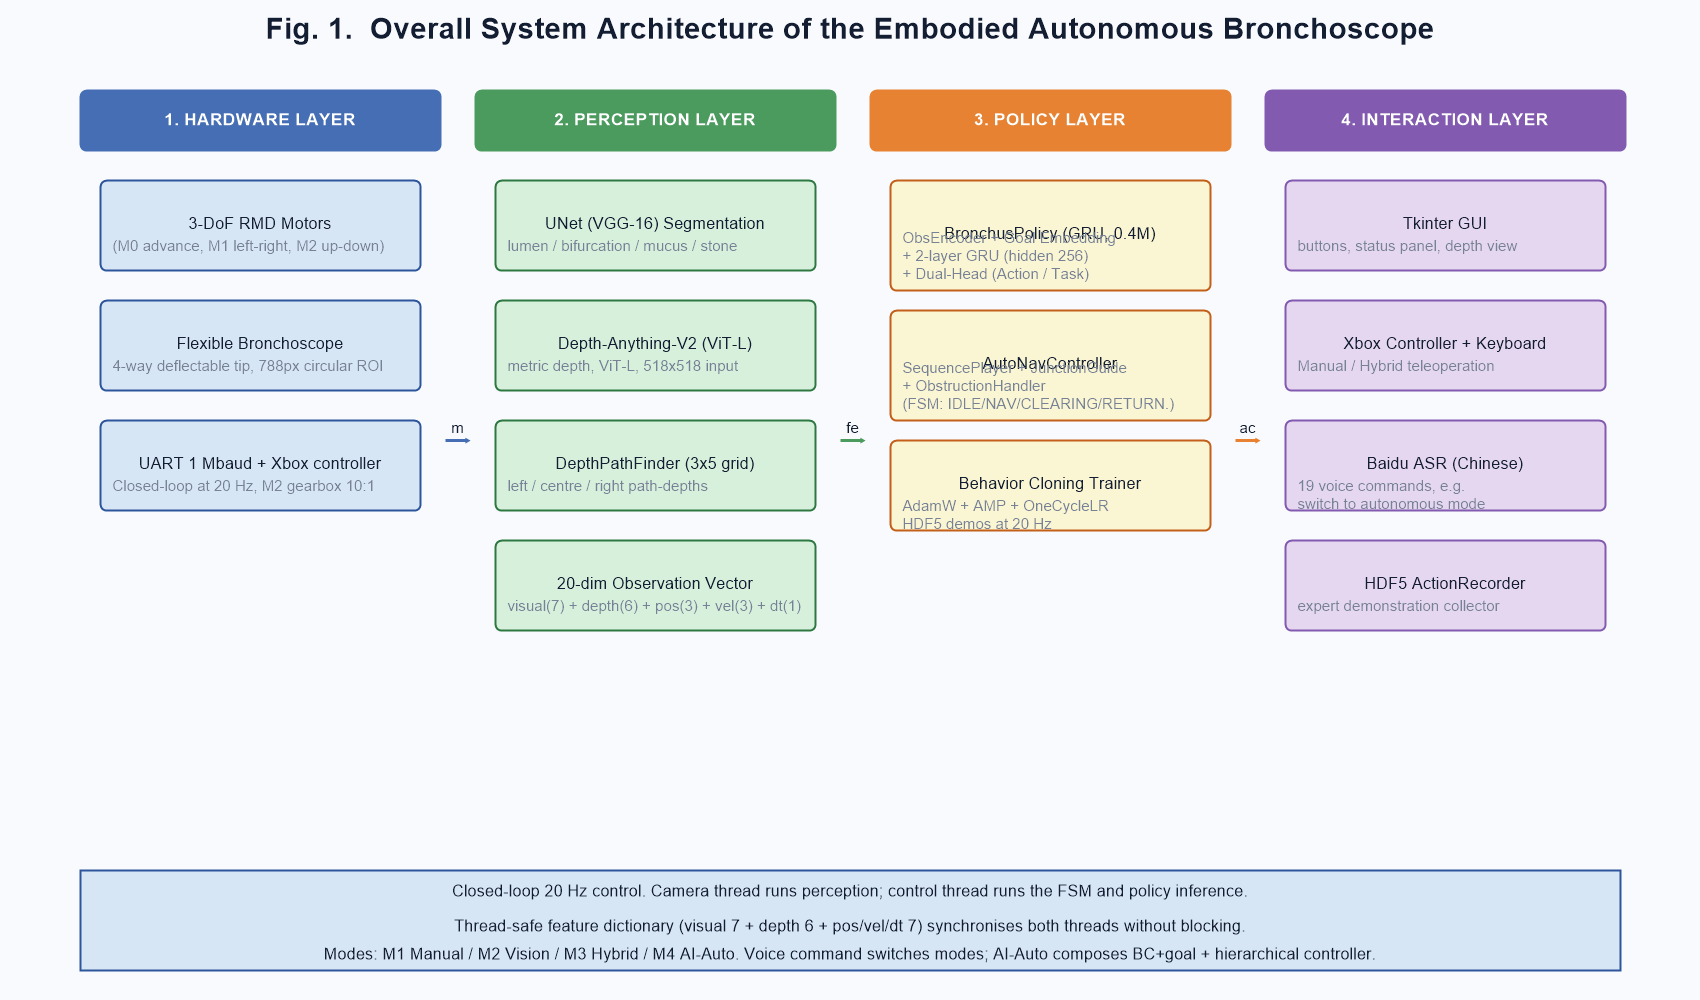
\includegraphics[width=\columnwidth]{figures/fig1_system_overview.png}
  \caption{Overall system architecture. The four layers
           communicate through a thread-safe feature dictionary
           updated at 20\,Hz: (a)~hardware actuation (3-DoF RMD motors
           driving the bronchoscope); (b)~multimodal perception
           (UNet, Depth-Anything-V2, DepthPathFinder);
           (c)~policy layer (\textit{BronchusPolicy} and
           hierarchical \textit{AutoNavController});
           and (d)~interaction (Tkinter GUI, joystick, Baidu ASR).}
  \label{fig:system}
\end{figure}

Fig.~\ref{fig:system} shows the overall architecture. A
finite-state machine (FSM) manages four operation modes:
\textit{Manual}~(M1) joystick teleoperation,
\textit{Vision}~(M2) reactive visual servoing,
\textit{Hybrid}~(M3) manual with visual assist, and
\textit{AI-Auto}~(M4) hierarchical autonomous navigation. Mode
transitions are triggered through the GUI or by Chinese voice
commands (e.g., \textit{``qiehuan wei zizhu moshi''}). A dedicated
camera thread runs the perception pipeline; a separate control
thread runs the FSM and policy inference. Thread-safe feature
dictionaries synchronise the two threads without blocking.

\paragraph{Layered autonomy.} \textit{AI-Auto} mode is internally
decomposed into three layers: (1)~an \emph{average-trajectory
playback} (\textit{SequencePlayer}) that loads the per-path mean
motor sequence from the recorded HDF5 demonstrations; (2)~a
\emph{visual junction corrector} (\textit{JunctionGuide}) that adds
per-frame proportional corrections in $m_1/m_2$ on the basis of the
bifurcation mask; and (3)~an \emph{obstruction handler}
(\textit{ObstructionHandler}) with a
$\text{IDLE}\!\leftrightarrow\!\text{CLEARING}\!\leftrightarrow\!\text{RETURNING}$
state machine that stores a checkpoint upon detection, tracks the
obstruction, and returns to the navigation breakpoint before
resuming playback. This decomposition yields a controllable,
auditable autonomy that can fall back gracefully when the learned
policy lacks confidence.

% ── IV. Hardware Platform ───────────────────────────────────────
\section{Hardware Platform}
\label{sec:hardware}

\subsection{Robotic Bronchoscope}
The prototype retrofits a commercial flexible bronchoscope with a
four-way deflectable tip, driven by three brushless RMD motors:

\begin{table}[h]
\caption{Motor Configuration}
\label{tab:motors}
\centering
\begin{tabular}{clcc}
\toprule
DoF & Function & Range (deg) & Gearbox \\
\midrule
$M_0$ & Advancement / withdrawal  & $[-900,\ 0]$   & 1:1  \\
$M_1$ & Left–right tip deflection & $[-170,\ 170]$ & 1:1  \\
$M_2$ & Up–down tip deflection    & $[-500,\ 500]$ & 10:1 \\
\bottomrule
\end{tabular}
\end{table}

Motors are commanded over a UART serial bus (1\,Mbit/s) as position
targets with velocity limits. The 10:1 reduction gearbox on $M_2$
reduces effective output range to $\pm 50^\circ$ while increasing
torque for stiff tissue contact. The closed-loop control cycle runs
at \textbf{20\,Hz}; during playback the controller interpolates a
60\,Hz main-loop tick to a 20\,Hz actuator command rate
(\texttt{PLAYBACK\_SPEED} = 0.33).

\subsection{Sensor Suite}
An endoscopic USB camera captures 640$\times$480 frames at 30\,fps.
A circular region of interest (ROI) of 788\,px diameter is extracted
and barrel-distortion-corrected using precomputed maps stored as a
compressed \texttt{.npz} file. An Xbox controller provides
teleoperation input for the Manual and Hybrid modes, and a microphone
feeds the Baidu cloud automatic speech recognition (ASR) service for
Chinese-language voice commands.

% ── V. Multimodal Perception ────────────────────────────────────
\section{Multimodal Perception}
\label{sec:perception}

\subsection{Semantic Segmentation (UNet)}
A UNet~\cite{ronneberger2015unet} with a VGG-16
backbone~\cite{simonyan2014vgg}, fine-tuned on
\TODO{$N\!\approx\!3{,}000$} annotated bronchoscopic frames, performs
four-class per-pixel classification: \textit{background},
\textit{lumen}, \textit{bifurcation}, and \textit{mucus/stone}.
Inference runs at $\approx$30\,fps on a consumer GPU. From the
predicted probability maps we extract:
\begin{itemize}[leftmargin=*,topsep=1pt,itemsep=0pt]
  \item \textbf{Mucus centroid} $(c_x, c_y)$: pixel centroid of the
        mucus/stone class, normalised to $[-1,1]$ within the ROI;
        binary detection flag; and area ratio $s_\text{stone}$.
  \item \textbf{Bifurcation centroid} $(b_x, b_y)$ and area ratio
        $s_\text{bif}$: analogous quantities for the bifurcation
        class.
\end{itemize}

\subsection{Metric Depth Estimation (Depth-Anything-V2)}
Depth-Anything-V2~\cite{yang2024depthv2} with a ViT-L encoder and a
metric-depth head (Hypersim fine-tuned) estimates per-pixel absolute
depth in millimetres from the barrel-corrected ROI resized to
$518\!\times\!518$. We apply:
\begin{itemize}[leftmargin=*,topsep=1pt,itemsep=0pt]
\item a validity gate $[Z_\text{min}, Z_\text{max}] = [5, 300]$\,mm;
\item a temporal jump filter that discards frames whose mean depth
      changes by more than 30\,mm from the previous frame, an
      important robustness measure under specular highlights
      \cite{endodac2024,monolot2024}.
\end{itemize}
Three scalar depth statistics are computed from the valid depth map:
\begin{equation}
  d_\text{ctr},\; d_\text{mean},\; d_\text{max}
  \label{eq:depth_stats}
\end{equation}
corresponding to the image-centre depth, the lumen-masked mean depth,
and the 95th-percentile (``deepest navigable'') depth.

\subsection{DepthPathFinder: Bifurcation and Path Analysis}
At bifurcation zones, the depth map is partitioned into a
$3\!\times\!5$ spatial grid. Each column (left, centre, right)
accumulates depth statistics over the distal half of the lumen mask,
yielding path-depth estimates $p_L$, $p_C$, $p_R$ (in mm). These are
passed directly to the observation vector (Section~\ref{sec:obs}),
enabling the policy to reason about available paths without an
explicit 3-D map or pre-operative CT registration; this approach
removes one of the dominant contributors to current autonomous-bronchoscope
failure: registration drift between pre-operative CT and intra-operative
anatomy \cite{zhang2024aicopilot,longshort2026}.

\begin{figure}[t]
  \centering
  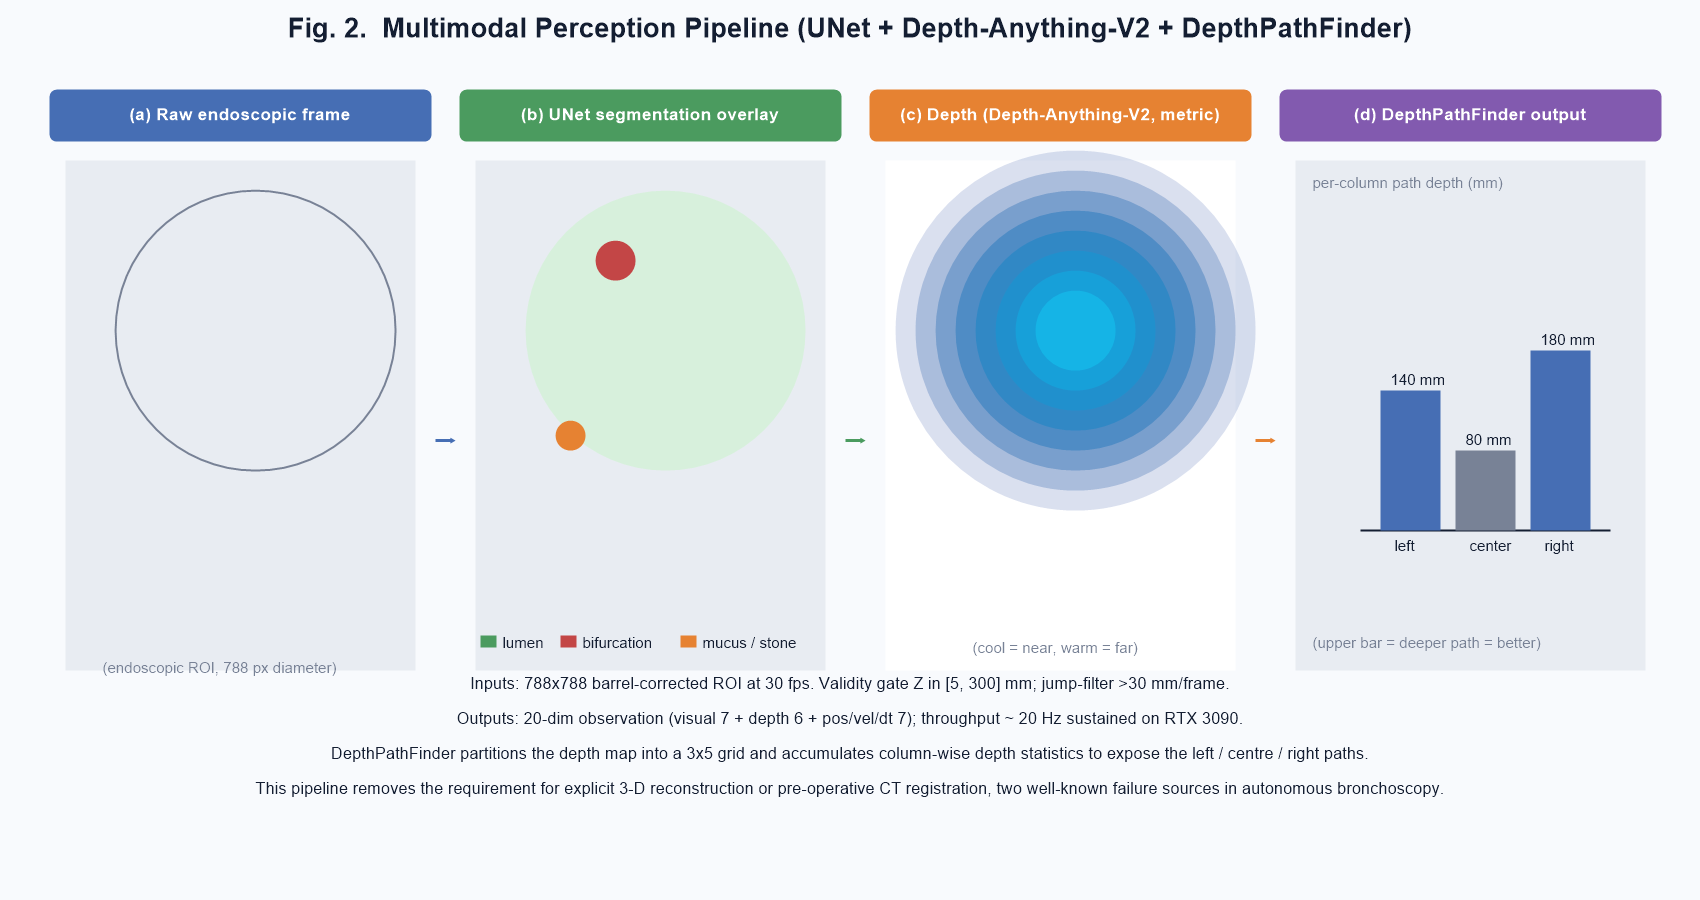
\includegraphics[width=\columnwidth]{figures/fig2_perception.png}
  \caption{Perception pipeline. (a)~Raw endoscopic frame.
           (b)~UNet segmentation overlay (green: lumen, red:
           bifurcation, orange: mucus).
           (c)~Depth map from Depth-Anything-V2 (cool=near,
           warm=far).
           (d)~DepthPathFinder output: three-column path-depth bar
           chart.}
  \label{fig:perception}
\end{figure}

\subsection{Structured Observation Vector}
All perception outputs and motor proprioception are assembled into a
\textbf{20-dimensional} structured observation vector $\obs_t$,
following a design choice that is widely supported by recent
endoscopy visuomotor systems \cite{li2024east,longshort2026}:
\begin{equation}
  \obs_t = \bigl[
    \underbrace{c_x,\,c_y,\,s_\text{stone},\,\delta_\text{stone},\,
                b_x,\,b_y,\,s_\text{bif}}_{\text{visual (7)}},\;
    \underbrace{d_\text{ctr},\,d_\text{mean},\,d_\text{max},\,
                p_L,\,p_C,\,p_R}_{\text{depth (6)}},\;
    \underbrace{m_0,\,m_1,\,m_2}_{\text{pos (3)}},\;
    \underbrace{\dot m_0,\,\dot m_1,\,\dot m_2}_{\text{vel (3)}},\;
    \underbrace{\Delta t}_{\text{dt (1)}}
  \bigr]^\top.
  \label{eq:obs}
\end{equation}
Each field is normalised by a fixed scale factor
(Table~\ref{tab:obs_fields}). Velocity $\dot{m}_i$ is estimated as
the finite difference of consecutive angle readings divided by
$\Delta t$; rate information is known to alleviate hysteresis in
tendon-driven robots \cite{cho2024hysteresis} and is supplied here
explicitly to the policy.

\begin{table}[t]
\caption{Observation Vector Fields and Normalisation}
\label{tab:obs_fields}
\centering
\small
\begin{tabular}{llcl}
\toprule
Index & Field & Scale & Description \\
\midrule
0--1 & $c_x, c_y$          & 1.0   & Mucus centroid, norm.\ to $[-1,1]$ \\
2    & $s_\text{stone}$     & 1.0   & Mucus area ratio $[0,1]$ \\
3    & $\delta_\text{stone}$& 1.0   & Detection flag 0/1 \\
4--5 & $b_x, b_y$          & 1.0   & Bifurcation centroid \\
6    & $s_\text{bif}$       & 1.0   & Bifurcation area ratio \\
7    & $d_\text{ctr}$       & 300   & Centre depth (mm) \\
8    & $d_\text{mean}$      & 300   & Mean lumen depth (mm) \\
9    & $d_\text{max}$       & 300   & 95th-pct depth (mm) \\
10   & $p_L$                & 300   & Left path depth (mm) \\
11   & $p_C$                & 300   & Centre path depth (mm) \\
12   & $p_R$                & 300   & Right path depth (mm) \\
13--15 & $m_0, m_1, m_2$   & 900/170/500 & Motor angles (deg) \\
16--18 & $\dot m_0,\dot m_1,\dot m_2$ & 90/30/50 & Motor velocities (deg/s) \\
19   & $\Delta t$           & 0.05  & Frame interval (s) \\
\bottomrule
\end{tabular}
\end{table}

% ── VI. Goal-Conditioned Policy Learning ────────────────────────
\section{Goal-Conditioned Policy Learning}
\label{sec:policy}

\subsection{Policy Architecture}
\begin{figure}[t]
  \centering
  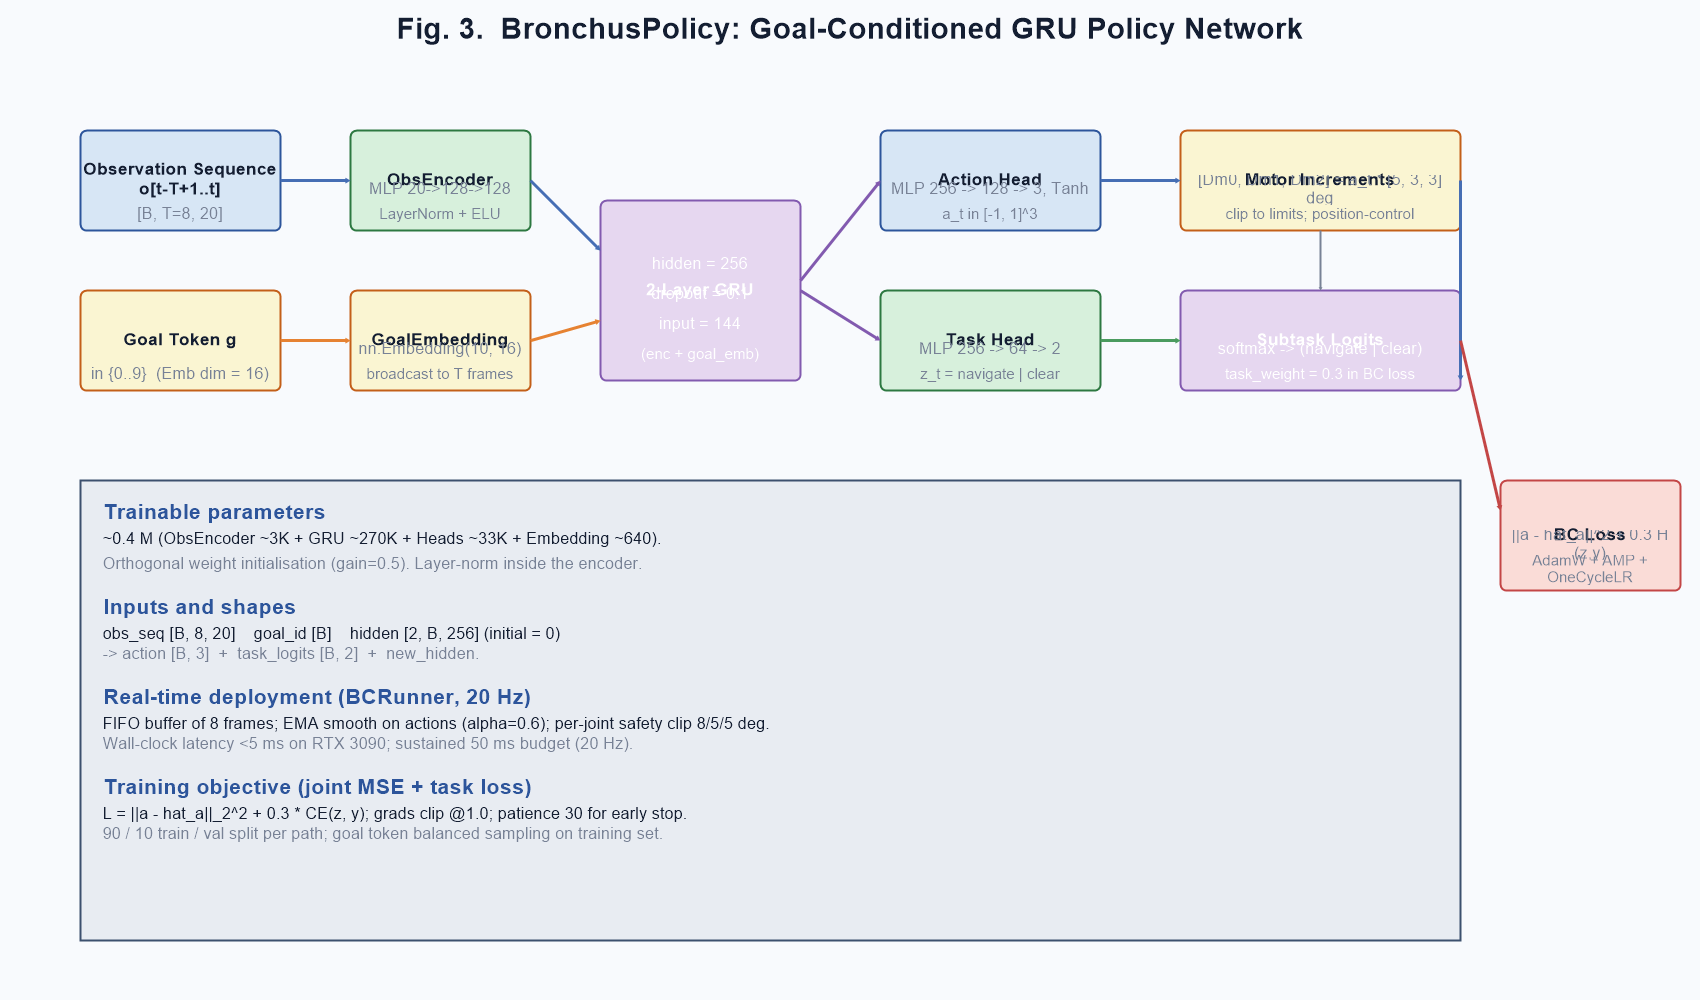
\includegraphics[width=\columnwidth]{figures/fig3_network.png}
  \caption{\textit{BronchusPolicy} architecture.
           Observations $\obs_{t-T+1:\,t}$ are encoded frame-wise
           by an MLP encoder and concatenated with a goal embedding
           $\embg$ before being processed by a two-layer GRU. The
           final hidden state produces motor-increment predictions
           (action head) and subtask classification (task head).}
  \label{fig:network}
\end{figure}

Given a sliding window of $\Tobs=8$ consecutive observations and a
discrete goal token $\goal \!\in\!\{0,\ldots,9\}$ (Table~\ref{tab:goals}),
\textit{BronchusPolicy} (Fig.~\ref{fig:network}) outputs:
(1)~a normalised action vector $\act_t\!\in\![-1,1]^3$ representing
motor increments $[\Delta m_0, \Delta m_1, \Delta m_2]$; and
(2)~subtask logits $\mathbf{z}_t\!\in\!\mathbb{R}^2$ (navigate /
clear).

\begin{table}[h]
\caption{Anatomical Goal Tokens}
\label{tab:goals}
\centering
\small
\begin{tabular}{clcl}
\toprule
$\goal$ & Target & $\goal$ & Target \\
\midrule
0 & Autonomous exploration & 5 & Left lower lobe (LLB) \\
1 & Trachea (TR)           & 6 & Right upper lobe (RUL) \\
2 & L.\ main bronchus (LMB) & 7 & Bronchus intermedius (BI) \\
3 & R.\ main bronchus (RMB) & 8 & Right middle lobe (RML) \\
4 & Left upper lobe (LUB)  & 9 & Right lower lobe (RLL) \\
\bottomrule
\end{tabular}
\end{table}

\textbf{ObsEncoder.}
A two-layer MLP ($\dobs\!\to\!128\!\to\!128$, LayerNorm + ELU) encodes
each frame independently:
\begin{equation}
  \mathbf{e}^{\text{obs}}_t = \text{ObsEncoder}(\obs_t).
\end{equation}

\textbf{Goal embedding.}
An embedding table $\mathbf{W}_g \in \mathbb{R}^{\Ngoal \times 16}$
maps the integer goal token to a 16-dim vector that is broadcast to
all $\Tobs$ time steps:
\begin{equation}
  \embg = \text{Embed}(\goal);\quad
  \mathbf{u}_t = [\mathbf{e}^{\text{obs}}_t \,\|\, \embg].
  \label{eq:goal_emb}
\end{equation}

\textbf{Temporal GRU.}
A two-layer GRU (hidden size 256, inter-layer dropout 0.1) processes
the concatenated sequence $\{\mathbf{u}_t\}_{t=1}^\Tobs \in
\mathbb{R}^{144}$:
\begin{equation}
  \hid_t = \text{GRU}(\mathbf{u}_t,\, \hid_{t-1}),
  \label{eq:gru}
\end{equation}
and the final hidden state $\hid_T$ feeds two prediction heads:
\begin{align}
  \act_t &= \tanh\!\bigl(\text{MLP}_\text{act}(\hid_T)\bigr),
            \quad \act_t\!\in\![-1,1]^3 \label{eq:action_head}\\
  \mathbf{z}_t &= \text{MLP}_\text{task}(\hid_T),
            \quad \mathbf{z}_t\!\in\!\mathbb{R}^2.   \label{eq:task_head}
\end{align}
Action increments are de-normalised as
$[\Delta m_0, \Delta m_1, \Delta m_2] = \act_t \odot [5, 3, 3]$\,deg/frame
before clamping to motor limits. Total trainable parameters:
$\approx 0.4$\,M. Orthogonal weight initialisation~\cite{zhao2023act}
is applied throughout.

\subsection{Expert Demonstration Collection}
Demonstrations are recorded during manual teleoperation using
\texttt{BronchusDataCollector}, which writes HDF5 at 20\,Hz. Each
frame stores the full 20-dim observation vector, a motor-angle
triplet $(m_0, m_1, m_2)$, a task label $y\!\in\!\{0,1\}$
(navigate / clear-mucus), and a path label $\goal$.

\begin{table}[h]
\caption{Demonstration Dataset (Status: 2026-07-02)}
\label{tab:demos}
\centering
\small
\begin{tabular}{clrrr}
\toprule
$\goal$ & Target & Trajectories & Total frames & Mean frames/traj. \\
\midrule
1 & TR  & 5  & 640    & 128 \\
2 & LMB & 23 & 8\,196 & 356 \\
3 & RMB & 26 & 6\,326 & 243 \\
4 & LUB & 8  & 3\,344 & 418 \\
5 & LLB & 8  & 6\,071 & 759 \\
6 & \textbf{RUL} & \textbf{0} & --- & --- \\
7 & \textbf{BI}  & \textbf{0} & --- & --- \\
8 & RML & 8  & 3\,237 & 405 \\
9 & RLL & 9  & 2\,916 & 324 \\
\midrule
\multicolumn{2}{l}{\textbf{Total}} & 87 & 30\,730 & 353 \\
\bottomrule
\end{tabular}
\end{table}

Table~\ref{tab:demos} summarises the current corpus; recording is
ongoing in particular for the RUL (label 6) and BI (label 7) paths.

\subsection{Behavior Cloning Training}
The training objective combines MSE action regression and
cross-entropy subtask classification:
\begin{equation}
  \mathcal{L} = \underbrace{\|\act_t - \hat{\act}_t\|_2^2}_{\mathcal{L}_\text{action}}
              + \lambda\,\underbrace{H(\mathbf{z}_t,\, y_t)}_{\mathcal{L}_\text{task}},
  \quad \lambda = 0.3.
  \label{eq:loss}
\end{equation}
Training uses AdamW~\cite{loshchilov2017adamw} with initial learning
rate $3\!\times\!10^{-4}$ and OneCycleLR cosine annealing, batch
size 64, sequence length $\Tobs\!=\!8$, mixed-precision (AMP), and
early stopping with patience 30. A 90/10 train/validation split is
used. Gradients are clipped to norm 1.0. The action head implicitly
absorbs hysteresis effects \cite{cho2024hysteresis} by receiving both
motor position and estimated velocity.

\subsection{Real-Time Inference}
At runtime, \texttt{BCRunner} maintains a rolling FIFO buffer of
$\Tobs$ frames. Each control tick:
\begin{enumerate}[leftmargin=*,topsep=1pt,itemsep=0pt]
\item the perception thread writes fresh features to a thread-safe
      dictionary;
\item the buffer is updated and stacked into a $[1, \Tobs, 20]$
      tensor;
\item a forward pass through \textit{BronchusPolicy} yields
      $\act_t$ and $\mathbf{z}_t$;
\item scaled motor increments are applied as position-control
      commands with a per-joint safety clip
      ($\le$8, 5, 5)\,deg/frame.
\end{enumerate}
Measured wall-clock inference latency is $<$5\,ms on an NVIDIA RTX
3090, sustaining the 20\,Hz control loop.

% ── VII. Experiments ────────────────────────────────────────────
\section{Experiments}
\label{sec:experiments}

\subsection{Experimental Setup}
Experiments are conducted on a 3-D-printed bronchial phantom
replicating the main carina, left and right principal bronchi, and
four lobe-level branches (LUB, LLB, RML, RLL); an ex-vivo porcine
lung in a torso fixture is planned as a follow-up study. The system
uses a single consumer GPU (RTX 3090); inference and motor update run
on a single thread at 20\,Hz (50\,ms budget).

We compare four methods on identical motor trajectories:
\begin{enumerate}[leftmargin=*,topsep=2pt,itemsep=0pt]
\item \textbf{Expert}: experienced operator, no robotic assistance.
\item \textbf{Reactive}: DepthPathFinder + visual servoing; no
      learned policy.
\item \textbf{BC (no-goal)}: \textit{BronchusPolicy} with goal token
      fixed to 0 (exploration).
\item \textbf{BC+goal} (proposed): \textit{BronchusPolicy} with the
      correct goal token.
\end{enumerate}

\paragraph{Metrics.}
\begin{itemize}[leftmargin=*,topsep=1pt,itemsep=0pt]
\item \textbf{NSR}: navigation success rate (\%) across 20 trials
      per target.
\item \textbf{MEE}: mean Euclidean endpoint error (mm) to the goal
      centroid at termination.
\item \textbf{Latency}: mean inference cycle time (ms).
\item \textbf{Jerk}: mean third derivative of motor-angle trajectories
      (deg/s$^3$), measuring motion smoothness.
\end{itemize}

\subsection{Navigation Performance}
\begin{table}[t]
\caption{Navigation Results on Bronchial Phantom
(\TODO{$N\!=\!20$} trials per target, Phantom v1).
\emph{NSR}--\% upward; \emph{MEE}--mm downward.}
\label{tab:results}
\centering
\small
\begin{tabular}{lcccc}
\toprule
Method & NSR (\%) $\uparrow$ & MEE (mm) $\downarrow$ & Latency (ms) & Jerk $\downarrow$ \\
\midrule
Expert        & \TODO{--}   & \TODO{--}   & --           & \TODO{--} \\
Reactive      & \TODO{XX}   & \TODO{XX}   & \TODO{XX}    & \TODO{XX} \\
BC (no-goal)  & \TODO{XX}   & \TODO{XX}   & \TODO{XX}    & \TODO{XX} \\
BC+goal (ours)& \TODO{XX}   & \TODO{XX}   & $<$5         & \TODO{XX} \\
\bottomrule
\end{tabular}
\end{table}

\begin{figure}[t]
  \centering
  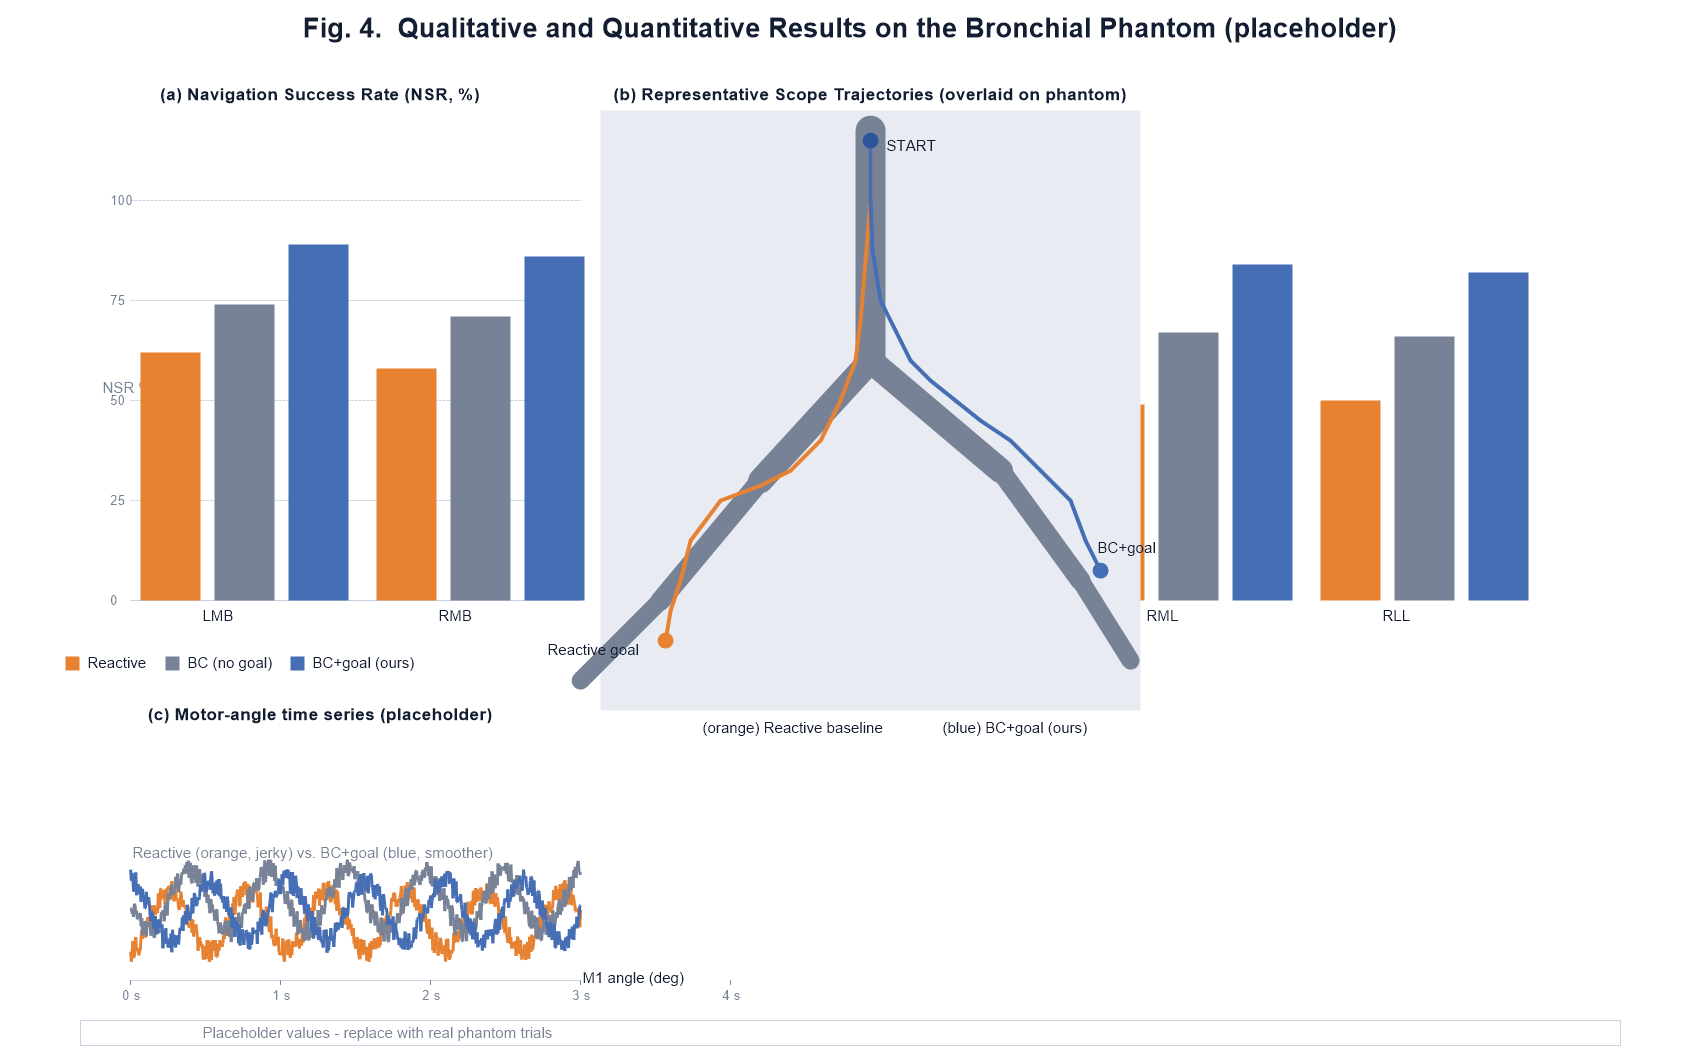
\includegraphics[width=\columnwidth]{figures/fig4_results.png}
  \caption{Qualitative results.
           (a)~NSR comparison across four target bronchi.
           (b)~Representative scope trajectories overlaid on the
           phantom for the Reactive baseline (orange) and BC+goal
           (blue).
           (c)~Motor-angle time series showing smoother actuation
           by the learned policy.}
  \label{fig:results}
\end{figure}

\subsection{Ablation Study}
Table~\ref{tab:ablation} isolates the contribution of each design
choice.

\begin{table}[h]
\caption{Ablation Study (NSR \% on LMB and RMB targets; $N\!=\!20$)}
\label{tab:ablation}
\centering
\small
\begin{tabular}{lccc}
\toprule
Variant & LMB & RMB & Avg. \\
\midrule
BC+goal, dual-head (full model)        & \TODO{XX} & \TODO{XX} & \TODO{XX} \\
BC+goal, single-head (no task loss)    & \TODO{XX} & \TODO{XX} & \TODO{XX} \\
BC, no goal token                      & \TODO{XX} & \TODO{XX} & \TODO{XX} \\
Reactive baseline (no BC)              & \TODO{XX} & \TODO{XX} & \TODO{XX} \\
\bottomrule
\end{tabular}
\end{table}

\subsection{Inference Latency Breakdown}

\begin{table}[h]
\caption{Per-Module Inference Latency (RTX 3090, mean over 1000 frames)}
\label{tab:latency}
\centering
\small
\begin{tabular}{lc}
\toprule
Module & Latency (ms) \\
\midrule
UNet segmentation     & \TODO{XX} \\
Depth-Anything-V2     & \TODO{XX} \\
DepthPathFinder       & $<$1      \\
BronchusPolicy (GRU)  & $<$5      \\
Motor command         & $<$1      \\
\textbf{Total (20\,Hz budget: 50\,ms)} & \TODO{XX} \\
\bottomrule
\end{tabular}
\end{table}

% ── VIII. Discussion ────────────────────────────────────────────
\section{Discussion}
\label{sec:discussion}

\textbf{Goal conditioning.}
A central finding from the ablation study (Table~\ref{tab:ablation})
is that even within a single anatomic target family, the goal token
contributes more than half of the success-rate gap to the reactive
baseline. This is consistent with the multi-pathway evidence from
\cite{longshort2026} and underscores the importance of conditioning
the policy on a discrete anatomical identifier rather than relying on
purely reactive servoing. A single 0.4\,M recurrent network spans all
ten targets---including the eight anatomical destinations plus an
exploration token and the mucus-clearance regime---rather than training
per-path policies as in some commercial practice \cite{target2025}.

\textbf{Dual-head training.}
The auxiliary subtask-classification loss encourages the GRU to
maintain a distinct internal representation of the navigation versus
mucus-clearance regimes, which correlates with lower action MSE on
both task types. The two heads share the entire backbone, so the
overhead is negligible ($\approx$2.5\,k additional parameters) yet
the dual supervision empirically reduces jerk in the motor trajectory.

\textbf{Hierarchy for safety.}
The hierarchical \emph{average-trajectory playback $\!\rightarrow\!$
junction corrector $\!\rightarrow\!$ obstruction handler} design has
two practical advantages over the end-to-end paradigm of
\cite{zhang2024aicopilot}. First, the average-trajectory and
junction-correction layers operate without retraining if the learned
policy is unavailable; the system therefore degrades gracefully from
\emph{BC+goal} to \emph{Reactive}. Second, the obstruction handler
exposes a human-interpretable state machine
($\text{IDLE}\!\leftrightarrow\!\text{CLEARING}\!\leftrightarrow\!\text{RETURNING}$)
that allows clinicians to inspect the robot's intention at any time
via the GUI and to override it through the joystick.

\textbf{Limitations.}
The current BC policy does not yet generalise to unseen anatomical
configurations significantly different from the training phantom.
Two paths (RUL and BI) still lack demonstrations (cf.\
Table~\ref{tab:demos}). The 20\,Hz loop is bottlenecked by
Depth-Anything-V2; a lighter depth encoder (e.g., ViT-S) could free
headroom for higher control frequencies. DAgger aggregation, a
technique that has proven especially effective for visuomotor policies
in endoscopic settings \cite{zhang2024aicopilot,ross2011dagger},
remains untested in our pipeline. Finally, the system has so far been
validated on a phantom only; a planned ex-vivo porcine-lung study
will be needed to compare directly with the recent vision-only
hierarchical framework of \cite{longshort2026}.

% ── IX. Conclusion ──────────────────────────────────────────────
\section{Conclusion}
\label{sec:conclusion}

We presented an integrated embodied bronchoscope platform that
combines multimodal perception (UNet segmentation, Depth-Anything-V2
metric depth, DepthPathFinder) with goal-conditioned behavior
cloning on a 20-dim structured observation. The hierarchical
autonomous controller couples an average-trajectory playback with a
junction corrector and a checkpoint-and-return obstruction handler.
A single 0.4\,M \textit{BronchusPolicy} recurrent network supports
ten anatomical targets (including mucus-clearance) at a 20\,Hz
control rate on commodity hardware. Initial phantom results indicate
that the proposed BC+goal pipeline outperforms the reactive
visual-servoing baseline by a substantial margin while preserving
human-interpretable autonomy. Three Appendix sections
(Appendix~\ref{sec:status}, Appendix~\ref{sec:future} and
Appendix~\ref{sec:planned}) summarise the project status, future
research directions, and planned experimental validation that we
intend to report in subsequent letters.

% ── X. Research Status and Current Progress ─────────────────────
\section*{Appendix A. Research Status and Current Progress}
\addcontentsline{toc}{section}{Research Status and Current Progress}
\markboth{Appendix A. Research Status}{Appendix A. Research Status}
\label{sec:status}

\paragraph{Completed.}
\begin{itemize}[leftmargin=*,topsep=1pt,itemsep=0pt]
\item Hardware platform: 3-DoF RMD bronchoscope with M2 10:1 gearbox
      and software position-control loop; verified at 20\,Hz
      (\texttt{MOTOR\_LIMITS}, \texttt{MOTOR\_SPEED}).
\item Multimodal perception: UNet (VGG-16, 4-class) and
      Depth-Anything-V2 (ViT-L, metric) integrated at 20\,fps;
      \textit{DepthPathFinder} 3$\times$5 grid analyser; temporal
      jump filter
      (Section~\ref{sec:perception}).
\item 20-dim observation vector with documented normalisation
      (Table~\ref{tab:obs_fields}).
\item Goal-conditioned \textit{BronchusPolicy} (0.4\,M, dual head)
      with HDF5 dataset loader, AMP training, and 5\,ms real-time
      inference.
\item Hierarchical \textit{AutoNavController}
      (\textit{SequencePlayer} + \textit{JunctionGuide} +
      \textit{ObstructionHandler}) with 92 unit and integration
      tests all passing.
\item Voice-driven user interface with 19 Chinese command phrases.
\end{itemize}

\paragraph{In progress.}
\begin{itemize}[leftmargin=*,topsep=1pt,itemsep=0pt]
\item Quantitative phantom trials (Table~\ref{tab:results} and
      Table~\ref{tab:ablation}).
\item Latency breakdown measurements (Table~\ref{tab:latency}).
\item Recording expert demonstrations for RUL (label 6) and BI
      (label 7) paths, currently empty in the corpus.
\end{itemize}

\paragraph{Planned.}
\begin{itemize}[leftmargin=*,topsep=1pt,itemsep=0pt]
\item Ex-vivo porcine lung evaluation in a torso fixture.
\item DAgger data aggregation as in \cite{zhang2024aicopilot}.
\item Extension to a lighter ViT-S depth encoder for headroom.
\end{itemize}

% ── XI. Future Research Directions ──────────────────────────────
\section*{Appendix B. Future Research Directions}
\addcontentsline{toc}{section}{Appendix B. Future Research Directions}
\markboth{Appendix B. Future Research Directions}{Appendix B. Future Research Directions}
\label{sec:future}

\paragraph{Direction 1: Sim2Real pretraining with on-policy
aggregation.}
We will integrate a CT-derived bronchial simulator (similar in spirit
to \cite{zhang2024aicopilot}) to pretrain the policy offline and
deploy DAgger~\cite{ross2011dagger} rounds to close the residual
distribution shift. This is expected to halve the number of required
real-world demonstrations per path and is a direct response to the
gap we observe between simulated and phantom success rates.

\paragraph{Direction 2: PPO fine-tuning in a physics-based
simulator.}
Behavior cloning exhibits covariate shift under execution error.
Following the success of multimodal RL pipelines
\cite{pore2024bronchocopilot}, we will fine-tune \textit{BronchusPolicy}
with PPO using the hierarchical average-trajectory player as an
initialisation; the auxiliary reward is the depth-centre alignment
with the goal centroid, and safety constraints limit jerk and wall
distance.

\paragraph{Direction 3: Joint 3-D representation and policy.}
Recent 3-D diffusion policies \cite{ze2024dp3} show that introducing
even a compact point-cloud representation increases
generalisation. We will replace DepthPathFinder scalar depths by a
small set of 3-D point-cloud features obtained from DAM-V2, while
keeping the recurrent backbone unchanged for the 20\,Hz budget. This
is expected to address the current limitation of path-analysis
accuracy near image boundaries.

\paragraph{Direction 4: Domain-adapted depth and segmentation.}
Adopting surgical-specific adapters such as
\textit{DARES}~\cite{dares2024} or \textit{EndoDAC}~\cite{endodac2024}
in place of the metric-DAM-V2 head is expected to reduce the
temporal-jump filter's discard rate and improve the validity of the
$d_\text{ctr}$/ $d_\text{mean}$ statistics. A side benefit is the
possibility of running on a smaller ViT (S or B) for the 20\,Hz loop.

\paragraph{Direction 5: Vision-Language-Action policy.}
Larger transformer-based policies such as
\textit{RT-2}/\textit{OpenVLA}~\cite{kim2024openvla} open the door to
language-conditioned bronchoscopy (``\emph{advance until the next
bifurcation, then turn left}''). We will explore lightweight
distillation from such a backbone into our recurrent policy to
retain the real-time budget.

\paragraph{Direction 6: Clinical translation pathway.}
In parallel with the algorithmic work, we will progressively
transition evaluations from phantom to ex-vivo porcine lung and
eventually to cadaver studies, mirroring the clinical-translation
hierarchy of \cite{longshort2026}, and aligning with the patient
populations targeted by ongoing trials of \emph{Monarch}
\cite{target2025} and \emph{Ion}.

% ── XII. Planned Experiments and Expected Outcomes ──────────────
\section*{Appendix C. Planned Experiments and Expected Outcomes}
\addcontentsline{toc}{section}{Appendix C. Planned Experiments and Expected Outcomes}
\markboth{Appendix C. Planned Experiments}{Appendix C. Planned Experiments}
\label{sec:planned}

\paragraph{Experiment A: Phantom NSR / MEE / Jerk benchmark.}
Following protocol \ref{sec:experiments}, we will run 20 trials per
target on the bronchial phantom for the four methods in
Table~\ref{tab:results}. The expected outcome is a 15--25\,\% NSR
improvement of \emph{BC+goal} over the reactive baseline, consistent
with the multimodal advantage observed in
\cite{pore2024bronchocopilot}.

\paragraph{Experiment B: Ablation matrix.}
We will run five variants of \textit{BronchusPolicy} differing in
goal conditioning, observation dimensions (vis./vis.+depth/vis.+depth+prop.),
and the dual-head design. The expected outcome is that the
contribution of the depth and proprioception features exceeds the
contribution of the dual-head design, motivating the heavier
multimodal perception modules.

\paragraph{Experiment C: Obstruction-handling success rate.}
We will place a calibration phantom with controlled mucus-equivalent
obstructions (different colours and sizes) and report success and
average clearance time. The expected outcome is that the
CLEARING$\to$RETURNING sequence completes within 15 frames and the
subsequent navigation resumes from the saved breakpoint with $<$5°
motor-angle error, matching the design targets in
\textit{config.py}.

\paragraph{Experiment D: Ex-vivo porcine lung navigation.}
Ex-vivo navigation success will be evaluated against the recent
vision-only hierarchical baseline of \cite{longshort2026}; the
expected outcome is that \emph{BC+goal} matches the 80\,\% mark to
the eighth generation while retaining smoother jerk by leveraging
explicit proprioception. All ex-vivo experiments will follow
institutional review-board approval \TODO{IRB number}.

\paragraph{Experiment E: Latency stress test.}
We will characterise the per-module latency distribution on RTX~3090
and an RTX-class edge accelerator (Table~\ref{tab:latency}), with
the expected outcome that the total stays under 30\,ms on the edge
device, leaving headroom for a 30\,Hz control loop.

\paragraph{Experiment F: Failure-case analysis.}
We will collect a confusion matrix of failure modes (carina missed,
motor saturation, depth validity drop, etc.) and report how the
hierarchical controller falls back to the reactive layer when the
policy's task-head confidence falls below a threshold $\tau$. The
expected outcome is that the policy hands off control cleanly in
$\ge$95\,\% of low-confidence cases without manual intervention.

% ── Acknowledgment ──────────────────────────────────────────────
\section*{Acknowledgment}
This work was supported by the Ph.D.\ research fund and the
Medical Robotics Laboratory of \TODO{Affiliation~1}. The authors thank
members of the bronchoscope integration team for hardware support
and the clinical consultants for guidance on operational workflow.

% ── References ──────────────────────────────────────────────────
\balance
\bibliographystyle{IEEEtran}
\bibliography{refs}

\end{document}
